%%%%%%%%%%%%%%%%%%%%%%%%%%%%%%%%%%%%%%%%%%%%%%%%%%%%%%%%%%%%%%%%%%%%%%%%%%%%%
%	E-Yantra, IIT-Bombay

%	Document Author: Bhumika Varshney
%	Date: 29- june-2015

%%%%%%%%%%%%%%%%%%%%%%%%%%%%%%%%%%%%%%%%%%%%%%%%%%%%%%%%%%%%%%%%%%%%%%%%%%%%%

\documentclass[10pt,red]{beamer} 
% change the alerted colour to blue
\setbeamercolor{alerted text}{fg=blue}

\usetheme{berlin}
% theme split
\usepackage{beamerthemesplit}

\usepackage{booktabs,array,}
\usepackage{listings}
\usepackage{hyperref}
\usepackage{verbatim,moreverb}
\usepackage{tikz}

\usepackage{color}

\definecolor{dkgreen}{rgb}{0,0.6,0}
\definecolor{gray}{rgb}{0.5,0.5,0.5}
\definecolor{mauve}{rgb}{0.58,0,0.82}

\lstset{frame=tb,
  language = Java,
  aboveskip=3mm,
  belowskip=3mm,
  showstringspaces=true,
  columns=flexible,
  basicstyle={\small\ttfamily},
  numbers=none,
  numberstyle=\tiny\color{gray},
  keywordstyle=\color{blue},
  commentstyle=\color{dkgreen},
  stringstyle=\color{mauve},
  breaklines=true,
  breakatwhitespace=true
  tabsize=4
}
% theme shadow
\usepackage{beamerthemeshadow}

% For including figures
\usepackage{graphicx}

% logo
\logo{
\includegraphics[height=1cm]{iitblogo.pdf}}


% sf family, bold font
\sffamily \bfseries
% Beginning of title page
\title
% content inside [] appears at bottom of all page. content inside {} appears on first page as title. double backslash means line change 
[
	Firebird LPC2148 Robotics Research Platform	% bottom
	\hspace{0.5cm}
	\insertframenumber/\inserttotalframenumber
]
{
	Basic IO Interfacing on Firebird-V 
}

\author
[
	www.e-yantra.org
]
{
	e-Yantra Team \\
  Embedded Real-Time Systems Lab\\
  Indian Institute of Technology-Bombay \\
}
\date
{
IIT Bombay \\ {\today}
}
 
 
\begin{document} 

% Slide-1: Title Page
\begin{frame}
	\titlepage
\end{frame} 

% Slide-2: Agenda for Discussion
\section*{Outline}
\begin{frame}
	\frametitle{Agenda for Discussion}
	\tableofcontents
\end{frame} 


\section{Input-Output Ports in LPC2148}
\subsection{Overview of Ports}
% Slide-3: Definition of PORTs
\begin{frame}
	\frametitle{What are Ports?} \pause
		\begin{enumerate}
			\item<+-|alert@+> Junctions where peripheral devices are connected. \\[10pt]
			\item<+-|alert@+> Peripheral devices can be  \\[10pt]
				\begin{enumerate}
				\item<+-|alert@+> Input Device  \\[10pt]
				 Example: Switch, Sensors, etc...\\[10pt]
				 \item<+-|alert@+> Output Device  \\[10pt]
				 Example: Buzzer,LCD,Motors,LED, etc...    
				\end{enumerate}
		\end{enumerate}
\end{frame}

% Slide-4: PORTs in LPC2148
\begin{frame}
	\frametitle{PORTS in LPC2148} \pause
		\begin{enumerate}
			\item<+-|alert@+> LPC stands for low power consumption.  \\[10pt]
			\item<+-|alert@+> LPC2148 is 64 pin controller  \\[10pt]
			\item<+-|alert@+> 44 pins can be used as Input/Output Pins  \\[10pt]
			\item<+-|alert@+> Pins are grouped together and called as PORT  \\[10pt]
			\item<+-|alert@+> LPC2148 has Two 32-bit ports  \\[10pt]
				 PORTx; \hspace{2cm} x = 0 or 1\\[10pt]
				\begin{enumerate}
				 \item<+-|alert@+> PORT 0- Out of 32 pins, 24th, 26th and 27th pins are not available and 31st pin can only be used as output pin.  \\[10pt]
				 \item<+-|alert@+> PORT 1- Out of 32 pins, 0 to 15 pins are not available.  \\[10pt]
				\end{enumerate}
		\end{enumerate}
\end{frame} 

\subsection{Acessing Ports}
% Slide-5: Acessing Ports
\begin{frame}
	\frametitle{Accessing PORTS} \pause
		\begin{enumerate}
			\item<+-|alert@+> Each Ports has five associated registers with it.   \\[10pt]
				\begin{enumerate}
					\item<+-|alert@+> PINSELx  \hspace{25pt} x = 0,1 and 2\\[10pt]
					\item<+-|alert@+> IOxDIR \hspace{30pt} x = 0 or 1\\[10pt]
					\item<+-|alert@+> IOxPIN \hspace{30pt} x = 0 or 1\\[10pt]    
					\item<+-|alert@+> IOxSET \hspace{30pt} x = 0 or 1\\[10pt]
					\item<+-|alert@+> IOxCLR \hspace{30pt} x = 0 or 1\\[10pt]
				\end{enumerate}
		\end{enumerate}
\end{frame} 

% Slide-6: Port Register PINSELx
\begin{frame}
	\frametitle{Understanding PINSELx Register} \pause
		\begin{enumerate}
			\item<+-|alert@+> Pin function Select Register   \\[10pt]
			\item<+-|alert@+> Purpose: To select the function of individual pins   \\[10pt]
			\item<+-|alert@+> PINSEL0 and PINSEL1 is used for PORT0  \\[10pt]
			\item<+-|alert@+> PINSEL2 is used for PORT1 \\[10pt]
			\item<+-|alert@+> Each pin can be used for atmost 4 functions so in PINSEL register 2 bits are provided for every single pin. \\[10pt]
		\end{enumerate}			
\end{frame}

% Slide-7: Port Register PINSELx
\begin{frame}
	\frametitle{Understanding PINSELx Register} \pause
	\begin{enumerate}
	\item<+-|alert@+> \color{red}PINSEL0 REGISTER\\[10pt] \color{black}
	\begin{tabular}{|c|c|c|c|c|c|c|c|c|c|}
		\hline D31 & D30 & D29 & D28 & ... & ... & D3 & D2 & D1 & D0 \\ 
		\hline
		\multicolumn{2}{|c|}{P0.15} & \multicolumn{2}{c|}{P0.14}& ... & ... & \multicolumn{2}{c|}{P0.1}  & \multicolumn{2}{c|}{P0.0}  \\ 
		\hline 
	\end{tabular}  	\pause
	\item<+-|alert@+> \color{red}PINSEL1 REGISTER\\[10pt] \color{black}
	\begin{tabular}{|c|c|c|c|c|c|c|c|c|c|}
		\hline D31 & D30 & D29 & D28 & ... & ... & D3 & D2 & D1 & D0 \\ 
		\hline
		\multicolumn{2}{|c|}{P0.31} & \multicolumn{2}{c|}{P0.30}& ... & ... & \multicolumn{2}{c|}{P0.17}  & \multicolumn{2}{c|}{P0.16}  \\ 
		\hline 
	\end{tabular} 	\pause
	\item<+-|alert@+> \color{red}PINSEL2 REGISTER\\[10pt] \color{black}
	\begin{tabular}{|c|c|c|c|c|c|c|c|c|c|}
		\hline D31 & D30 & D29 & D28 & ... & ... & D3 & D2 & D1 & D0 \\ 
		\hline
		\multicolumn{2}{|c|}{P1.31} & \multicolumn{2}{c|}{P1.30}& ... & ... & \multicolumn{2}{c|}{P1.17}  & \multicolumn{2}{c|}{P1.16}  \\ 
		\hline 
	\end{tabular} \pause	
	\end{enumerate}			
\end{frame}

% Slide-8: Port Register PINSELx
\begin{frame}
	\frametitle{Understanding PINSELx Register} \pause
	\begin{itemize}
		\item<+-|alert@+> For Example-    \\[10pt]
		Consider P0.0 pin- to select function for P0.0 we require D0 and D1 of PINSEL0 register.
	\pause
	\begin{center}
	\begin{tabular}{|c|c|}
		\hline \textbf{D1 D0} & \textbf{Function} \\ 
		\hline 00 & GPIO \\ 
		\hline 01 & UART0(TxD) \\ 
		\hline 10 & PWM1 \\ 
		\hline 11 & Reserved \\ 
		\hline 
	\end{tabular} \pause
	\end{center}
		\item<+-|alert@+> To set all pins of PORT 0 as GPIO, \\
			PINSEL0= 0x00000000;\hspace{0.8cm}\color{red}To set P0.0 to P0.15 pins as GPIO\color{black} \\
			PINSEL1= 0x00000000;\hspace{0.8cm}\color{red}To set P0.16 to P0.31 pins as GPIO\color{black} \\
	\end{itemize} 			
\end{frame}

% Slide-9: IOxDIR Register
\begin{frame}
	\frametitle{Understanding IOxDIR Register} \pause
		\begin{enumerate}
			\item<+-|alert@+> GPIO port direction control register   \\[10pt]
			\item<+-|alert@+> Purpose: To control the direction of each port pin    \\[10pt]
			\begin{itemize}
				\item<+-|alert@+> IOxDIR=0 ; PORTx is defined as INPUT  \\[10pt]	
				\item<+-|alert@+> IOxDIR=1 ; PORTx is defined as OUTPUT  \\[10pt]
			\end{itemize}			
			\item<+-|alert@+> \color{red}Example: \\[10pt]
		\color{black}For Port0 make lower word as input and upper word as
			output  \\[10pt]
			\pause	
			PINSEL0=0x00000000; \\
			PINSEL1=0x00000000;\\
			IO0DIR=0xFFFF0000;
		\end{enumerate}
\end{frame}

% Slide-10: IOxPIN Register
\begin{frame}
	\frametitle{Understanding IOxPIN Register} \pause
	\begin{enumerate}
		\item<+-|alert@+> GPIO port pin value register   \\[10pt]
		\item<+-|alert@+> Purpose: To read the current status of port and to write data on port regardless of the pin direction  \\[10pt]
		\item<+-|alert@+> Save value of a register in a variable  \\[10pt]			
		\item<+-|alert@+> \color{red}Example: Read data from Port0  \\[10pt]
		\pause	\color{black}
		Suppose value of PORT0 is 0xFFFF0000 \\ \pause
		x=IO0PIN; \\ \pause
		then x=0xFFFF0000 \pause
	\end{enumerate}
\end{frame}

% Slide-11: IOxSET Register 
\begin{frame}
	\frametitle{Understanding IOxSET Register} \pause
		\begin{enumerate}
			\item<+-|alert@+> GPIO port output set register\\[10pt]
			\item<+-|alert@+> Purpose: To set logic 1 on desired pins   \\[10pt]
			\item<+-|alert@+> Writing ones produces highs at the corresponding port pins, writing zeroes has no effect.\\[10pt]
			\item<+-|alert@+> \color{red}Example: To set bit 0 of PORT0(P0.0),  \\[10pt] \pause
			\color{black} 
			IO0SET=0x00000001; \\[10pt] \pause
			Suppose value of PORT0 was 0xFFFF0000, then after execution of the above instruction, value of PORT0 will be 0xFFFF0001 \pause
		\end{enumerate}
\end{frame}

% Slide-12: IOxCLR Register 
\begin{frame}
	\frametitle{Understanding IOxCLR Register} \pause
	\begin{enumerate}
		\item<+-|alert@+> GPIO port output Clear register\\[10pt]
		\item<+-|alert@+> Purpose: To set logic 0 on desired pins   \\[10pt]
		\item<+-|alert@+> Writing ones produces lows at the corresponding port pins, writing zeroes has no effect.\\[10pt]
		\item<+-|alert@+> \color{red}Example: To reset bit 31 of PORT0(P0.31),  \\[10pt] \pause
		\color{black} 
		IO0CLR=0x80000000; \\[10pt] \pause
		Suppose value of PORT0 was 0xFFFF0000, then after execution of the above instruction, value of PORT0 will be 0x7FFF0000 \pause
	\end{enumerate}
\end{frame}

\subsection{Example}
% Slide-13: Example
\begin{frame}
	\frametitle{Example}
	\begin{enumerate}
		\item<+-|alert@+> Example: Make PORT0 as output port and send bit pattern of 0000FFFF	\\[5pt]	\pause
		\begin{itemize}
			\item<+-|alert@+> Step 1: Select Port 0 as GPIO port \\[5pt]
			\ \ \	PINSEL0=0x00000000; \\
			\ \ \	PINSEL1=0x00000000; \\[5pt] \pause
			\item<+-|alert@+> Step 2: Make PORT0 as output port	\\[5pt]
			\ \ \ IO0DIR=0xFFFFFFFF; \\[5pt] \pause
			\item<+-|alert@+> Step 3: Put data on the Port 0 \\[5pt]
			\ \ \ IO0SET=0x0000FFFF; \\ 
			\ \ \ IO0CLR=0xFFFF0000; \\[5pt] \pause
			\ \ \ \ \ \ OR \\[5pt]
			\ \ \ IO0PIN=0x0000FFFF; \pause
		\end{itemize} 	
	\end{enumerate}
\end{frame}
% Slide-14 : C Program
\section{Write Your First Embedded C Program}
\subsection{Buzzer Interfacing}
\begin{frame}
	\frametitle{Buzzer Interfacing in Firebird V}	\pause
		\begin{enumerate}
			\item<+-|alert@+> Buzzer Connected to Port0 pin 25 	\pause\\[10pt]
				\hspace{3cm}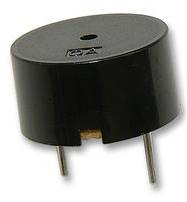
\includegraphics[width=0.5\linewidth]{buzzer}	\pause\\[10pt]
			\item<+-|alert@+>  To Turn on buzzer: \pause send logic HIGH on pin25 of Port0 \pause\\[10pt]
			\item<+-|alert@+>  To Turn off buzzer: \pause send logic LOW on pin25 of Port0
		\end{enumerate}
\end{frame}
% Slide-15 : Buzzer Program
\begin{frame}
	\frametitle{Buzzer Program}	\pause
		\begin{enumerate}
			\item<+-|alert@+> Set P0.25 as GPIO\pause\\[10pt]
			\ \ \ PINSEL1= 0x00000000; \pause\\[10pt]
			\item<+-|alert@+> Configure PORT0.25 pin as output.\pause\\[10pt]
				\ \ \ IO0DIR= 0x02000000;  \pause\\[10pt]
 			\item<+-|alert@+> To turn ON the buzzer set P0.25 output high\pause\\[10pt]
			 IO0SET = 0x02000000;\pause\\[10pt]
			\item<+-|alert@+> To turn OFF the buzzer set P0.25 output low\pause\\[10pt]
			 IO0CLR = 0x02000000;\pause\\[10pt]
		\end{enumerate}
\end{frame}
% Slide-16 : Programming Tools
\subsection{Programming Tools}

\begin{frame}
	\frametitle{ARM Programming Tools}	\pause
		\begin{enumerate}
			\item <+-|alert@+> Software Required.\pause\\[10pt]
				Keil uVision4 \pause\\[10pt]
				\item[$\bullet$]Integrated Development Environment (IDE) \\
				\item[$\bullet$]Supports Developing and Debugging of ARM based microcontroller application\\ 
				
			\item [$\bullet$] Download Link: \url{http://www.keil.com/arm/mdk.asp}  \pause\\[10pt]
 			\item <+-|alert@+> Hardware Required\pause\\[10pt]
			 
			\item[$\bullet$] hex file can be loaded into microcontroller using \pause\\
			\begin{enumerate}[a.]
				\item<+-|alert@+>	BootLoader\pause
				\item<+-|alert@+>	ARM Programmers viz. FlashMagic, LPC2000 Flash Utility, winARM etc..	
			\end{enumerate}
		\end{enumerate}
\end{frame}
% Slide-17 : C-code
\subsection{C-code}

\begin{frame}[shrink = 2,fragile] 
	\frametitle{Syntax for C-Program}\pause
	
		\begin{block}<1->{\#include}\pause
		\begin{semiverbatim}
				#include <lpc214x.h>
 		\end{semiverbatim}
		\end{block} \pause
		
	\begin{block}<2->{Pin Configuration}\pause
		\begin{semiverbatim}
				void Init_buzzer_pin (void)
				\{
 			 \ \ \		PINSEL1 = 		
 			 \ \ \		IO0DIR =
			 \ \ \ \ \		IO0CLR =  	\color{red}{\\\\ Initially buzzer off}\color{black}
				\}
 		\end{semiverbatim}
		\end{block}	
\end{frame}

% Slide-18 : Main Program
\begin{frame}[shrink = 4,fragile]
	\frametitle{Syntax for C-Program} \pause
	
		\begin{block}<1->{Main-Program}	\pause
		\begin{semiverbatim}
				int main (void) 
				\{
			\ \		 Init_buzzer_pin ();
			\ \		 while(1)
			\ \	 	\{
			\ \ \ \ \ \				buzzer_on();
			\ \ \ \ \ \				delay_ms();
			\ \ \ \	\ \			buzzer_off();
			\ \ \ \	\ \			delay_ms();
			\ \	 	\}	
				\}	
			\end{semiverbatim}
		\end{block} \pause
	
	\begin{block}<2->{Functions}\pause
		\begin{semiverbatim}
				void buzzer_on (void)
				\{
 		\ \ \		IO0SET = 0x02000000;		
				\}
				
				\hrule \hrule	\pause
				void buzzer_off (void)
				\{
 		\ \ \		IO0CLR = 0x02000000;		
				\}
 		\end{semiverbatim}
	\end{block}
		
\end{frame}
% Slide-19 : Thank You
\begin{frame}
\hskip4cm
\textbf{\LARGE Thank You!} \\[20pt]
\hskip3cm
\scriptsize Post your queries on: 
\hyperref[www.e-yantra.org]{\color{blue} http://qa.e-yantra.org/ \color{black}} 
\end{frame}
\end{document} 